\documentclass{beamer}

\usepackage[utf8]{inputenc}
\usepackage[spanish]{babel}
\usepackage{graphicx}

\setlength{\parskip}{1em}
\setlength{\parindent}{1em}

\xdefinecolor{rojito}{rgb}{1,0.3,0.3}
\xdefinecolor{oliva}{cmyk}{0.64,0,0.95,0.4}
\xdefinecolor{minaranja}{rgb}{0.94,0.48,0.2}

\usetheme{Madrid}
\usecolortheme[named=rojito]{structure}

% Para circuitos cuanticos. Requiere tener en el directorio el archivo qcircuit.sty
\usepackage{qcircuit}

\usepackage{mathtools}
\usepackage{amsmath}
%------------------------
%------- TEOREMAS -------
%------------------------

\newtheorem{thm}{Teorema} % Estilo de texto cursivo

\newtheorem{postulate}{Postulado} % Numeración general sin subíndices

\title[Computación Cuántica con Qiskit]{Introducción a la Computación Cuántica con Qiskit}
\author{Javier Pellejero Ortega}
\institute[UCM]{Universidad Complutense de Madrid\\ Facultad de Matemáticas}

% Conjuntos y constantes matemáticas
\newcommand{\R}{\mathbb{R}} % Reales
\newcommand{\C}{\mathbb{C}} % Complejos
\newcommand{\K}{\mathbb{K}} % Cuerpo K (reales o complejos)
\newcommand{\Sp}{\mathbb{S}} % Esfera
\newcommand{\e}{\mathrm{e}} % número e
\newcommand{\N}{\mathbb{N}} % Naturales
\newcommand{\Q}{\mathbb{Q}} % Racionales
\newcommand{\B}{\mathcal{B}} % Base

\newcommand{\qsh}{\textsf{Q}\texttt{\#}} % Q#
\newcommand{\csh}{\textsf{C}\texttt{\#}} % C#

\newcommand{\orden}[1]{\mathcal{O}\left(#1\right)}

\newcommand{\oversim}[1]{\overset{_\sim}{#1}} % Para poner ~ sobre algo

% Para poner datos encima y/o debajo de implica
\newcommand{\ximplies}[2]{\underset{#2}{\overset{#1}\implies}}
\newcommand{\xiff}[2]{\underset{#2}{\overset{#1}\iff}}
\newcommand{\ximpliedby}[2]{\underset{#2}{\overset{#1}\impliedby}}

% Producto escalar y norma
\newcommand{\dotproduct}[2]{\langle#1,#2\rangle}
\newcommand{\norm}[1]{\left|\left|#1\right|\right|}

% Notación de Dirac -- SUSTITUIR POR PAQUETE DE LUIS
\newcommand{\ket}[1]{\left|#1\right\rangle}
\newcommand{\bra}[1]{\left\langle#1\right|}
\newcommand{\braket}[2]{\left\langle#1|#2\right\rangle}

% Vectores
\newcommand{\twovector}[2]{\begin{pmatrix} #1 \\ #2 \end{pmatrix}} % Vector de dim 2

% Funciones e info debajo de funciones
\newcommand{\function}[3]{#1\colon #2\longrightarrow #3}
\newcommand{\xfunction}[4]{\underset{#4}{{#1\colon #2\longrightarrow #3}}}

% Funcion que transforma estados |0> y |1>
\newcommand{\gatetwo}[3]{#1\colon \begin{matrix}\ket0&\longrightarrow& #2\\ \ket1&\longrightarrow& #3\end{matrix}}

% Funcion que transforma estados |00>, |01>, |10> y |11>
\newcommand{\gatefour}[5]{#1\colon \begin{matrix} \ket{00}&\longrightarrow& #2\\ \ket{01}&\longrightarrow& #3\\ \ket{10}&\longrightarrow& #4\\ \ket{11}&\longrightarrow& #5 \end{matrix}}

% Para código
\usepackage{listings}
%\usepackage[table,xcdraw]{xcolor} % tambíen incluye colores para tablas.

\definecolor{codegreen}{rgb}{0,0.6,0}
\definecolor{codegray}{rgb}{0.5,0.5,0.5}
\definecolor{codepurple}{rgb}{0.58,0,0.82}
\definecolor{backcolour}{rgb}{0.95,0.95,0.92}

\lstdefinestyle{mystyle}{
    backgroundcolor=\color{backcolour},   
    commentstyle=\color{codegreen},
    keywordstyle=\color{magenta},
    numberstyle=\tiny\color{codegray},
    stringstyle=\color{codepurple},
    basicstyle=\ttfamily\footnotesize,
    breakatwhitespace=false,         
    breaklines=true,                 
    captionpos=b,                    
    keepspaces=true,                 
    numbers=left,                    
    numbersep=5pt,                  
    showspaces=false,                
    showstringspaces=false,
    showtabs=false,                  
    tabsize=2
}

\lstset{style=mystyle}

\begin{document}

\begin{frame}
	\titlepage
	\begin{center} Doble Grado en Matemáticas e Ingeniería Informática\end{center}
\end{frame}

\begin{frame}
\frametitle{Índice}
	\tableofcontents
\end{frame}

\section{Espacios de Hilbert}
\begin{frame}
	\frametitle{Espacio de Hilbert}
	\begin{itemize}
		\item  Un \emph{espacio de Hilbert} es un espacio vectorial dotado de producto interno y cuyo espacio normado definido por la norma
		$$\norm{x}\coloneqq\sqrt{\dotproduct{x}{x}}$$
es completo.
		\item En particular, $\C$ es un espacio de Hilbert con el producto interno $\dotproduct{x}{y}=x\overline{y}$ y lo mismo podemos decir de $\C^n$ con el producto interno $\dotproduct{x}{y}=\sum_{i=1}^n x_i\overline{y_i}$.
	\end{itemize}
\end{frame}

\subsection*{Isomorfismos lineales}
\begin{frame}
	\frametitle{Aplicaciones lineales}
	\begin{itemize}
		\item  Sean $V$ y $W$ dos espacios vectoriales sobre un cuerpo $\K$. $\function{f}{V}{W}$ es una \emph{aplicación lineal} si verifica
		$$f(\alpha x+ \beta y)= \alpha f(x)+\beta f(y)$$
		para todo $\alpha,\beta\in\K$ y para todo $x,y\in V$.
		\item Una aplicación lineal está totalmente determinada por su matriz asociada perteneciente a $\mathfrak{M}_{m,n}(\K)$ donde $m$ es la dimensión del espacio de entrada $V$ y $n$ la dimensión del espacio de salida $W$.
		\item Si $A$ es la matriz asociada a la aplicación lineal $f$ se verifica
		$$Ax=y \textrm{ para todos }x\in V \textrm{ e } y\in W$$
	\end{itemize}
\end{frame}

\begin{frame}
	\frametitle{Isomorfismos lineales en espacios de Hilbert}
	\begin{itemize}
		\item Nosotros estamos interesados en isomorfismos lineales sobre espacios de Hilbert.
		\item Un isomorfismo lineal $f$ con matriz asociada $U$ es \emph{unitario} si verifica $UU^\dag=I$. $U^\dag$ es la matriz adjunta de $U$ ($U^\dag=\overline{U}^t$) y además está asociada al isomorfismo adjunto de $f$ que es aquel que verifica
		$$\dotproduct{x}{Uy}=\dotproduct{U^\dag x}{y}$$
		\item Las matrices unitarias preservan el producto interno y, por tanto, la ortonormalidad.
		$$\dotproduct{Ux}{Uy}=(Ux)^t\overline{Uy}=x^tU^t\overline{U}\overline{y}=x^tI\overline{y}=\dotproduct{x}{y}$$
		Luego si $x\perp y$, entonces $Ux\perp Uy$.
	\end{itemize}
\end{frame}



\subsection*{Producto tensorial}

\begin{frame}
	\frametitle{Producto tensorial}
	\begin{itemize}
		\item El producto tensorial de dos espacios de Hilbert $V$ y $W$ con bases ortonormales $\B_V$ y $\B_W$, respectivamente, es el espacio de Hilbert $V\otimes W$ con base ortonormal dada por el conjunto $$\B=\{v\otimes w:v\in\B_V,w\in\B_W\}$$
		\item Sean $m$ y $n$ las dimensiones de $V$ y $W$ respectivamente, el espacio $V\otimes W$ generado tiene dimensiones $mn$.
		\item Dotamos a $V\otimes W$ de estructura de espacio de Hilbert con el producto interno definido por
		$$\dotproduct{v_1\otimes w_1}{v_2\otimes w_2}=\dotproduct{v_1}{v_2}_V\dotproduct{w_1}{w_2}_W,\ v_1,v_2\in V,\ w_1,w_2\in W$$
		siendo $\dotproduct{\cdot}{\cdot}_V$ el producto interno de $V$ y $\dotproduct{\cdot}{\cdot}_W$ el de $W$.
	\end{itemize}
\end{frame}

\section{Postulados cuánticos}

\subsection*{Postulados}
\begin{frame}
	\frametitle{Primer postulado. Sistemas cuánticos}
	
	\begin{postulate} Un sistema físico aislado es un espacio vectorial con coeficientes en los complejos dotado de producto interno, es decir, un espacio de Hilbert complejo. El sistema es completamente descrito por un estado que no es más que un vector unitario de dicho sistema.
\end{postulate}
\end{frame}

\begin{frame}
	\frametitle{Segundo postulado. Evolución de un sistema cuántico}
	
	\begin{postulate} La evolución de un sistema cuántico cerrado en dos instantes de tiempo viene dada por una transformación lineal unitaria. Es decir, el estado del sistema $\ket{\psi}$ en el instante~$t_1$ se transforma en $\ket{\psi'}$ en~$t_2$ por la aplicación lineal unitaria $U$ que depende únicamente de $t_1$ y $t_2$:
\[\ket{\psi'}=U\ket{\psi}\]
\end{postulate}
\end{frame}

\begin{frame}
	\frametitle{Tercer postulado. Medición de un sistema cuántico}
	
	\begin{postulate} Las medidas de un sistema cuántico son descritas por un conjunto $\{M_m \}$ de \textit{aplicaciones de medida}. Cada índice $m$ se identifica con un posible valor de medición $\ket\psi$. Se verifica:
	
	\begin{itemize}
	\item Probabilidad $p(m)=\bra{\psi}M_m^\dag M_m\ket{\psi}$
	\item Estado tras la medición $\dfrac{M_m\ket{\psi}}{\sqrt{\bra{\psi}M_m^\dag M_m\ket{\psi}}}=e^{i\theta}\ket\psi\overset{\textcolor{red}{!!}}=\ket\psi$
	\item Ecuación de completitud $\sum_m M_m^\dag M_m = I$
	\item La suma de probabilidades es 1. $\sum_m p(m)=\sum_m \bra{\psi}M_m^\dag M_m\ket{\psi} = 1$
	\end{itemize}
\end{postulate}
\end{frame}

\begin{frame}
	\frametitle{Cuarto postulado. Composición de sistemas cuánticos}
	
	\begin{postulate} El sistema resultante de la composición de dos o más sistemas físicos es el producto tensorial de los mismos. Si denotamos a estos sistemas por $1,2,...,n$ representados por los vectores unitarios $\ket{\psi_i}$ para todo $i=1,2,...,n$, entonces el estado del sistema final total es:
	$$\ket{\psi_1}\otimes\ket{\psi_2}\otimes\hdots\otimes\ket{\psi_n}$$
\end{postulate}
\end{frame}

\subsection*{Consecuencias de los postulados}
\begin{frame}
	\frametitle{Primer postulado. Qubit}
	
	\begin{itemize}
	\item El \emph{qubit} será nuestro elemento de información mínima.
	\item Vector unitario de $\C^2$. Tomando la base ortonormal $\{\ket0,\ket1\}$ (normalmente asociada a la base canónica) podemos escribir cualquier estado cuántico como
	$$\ket\psi=\alpha\ket0+\beta\ket1\textrm{ con }|\alpha|^2+|\beta|^2=1$$
	\end{itemize}
\end{frame}

\begin{frame}
	\frametitle{Tercer postulado. Mediciones}
	
	\begin{itemize}
	\item Aplicaciones de medida $M_{\ket{0}}\coloneqq\left(\begin{matrix}1&0\\0&0\end{matrix}\right)$ y $M_{\ket{1}}\coloneqq\left(\begin{matrix}0&0\\0&1\end{matrix}\right)$.
	\item Para $\ket\psi=\alpha\ket0+\beta\ket1$, $p(\ket0)=|\alpha|^2$ y $p(\ket1)=|\beta|^2$.
	\item El estado tras la medición es:
		$$\dfrac{\alpha}{|\alpha|}\ket0\overset{\textcolor{red}{!!}}=\ket0\textrm{ o }\dfrac{\beta}{|\beta|}\ket1\overset{\textcolor{red}{!!}}=\ket1$$
	\item Se verifica la ecuación de completitud: $M_{\ket{0}} + M_{\ket{1}}=I$.
	\item $p(\ket0)+p(\ket1)=1$.
	
	\end{itemize}
\end{frame}

\begin{frame}
	\frametitle{Cuarto postulado. Sistemas de múltiples qubits}
	
	\begin{itemize}
	\item Un sistema de $n$ qubits vendrá representado por un vector unitario de $\C^{2^n}$.
	\item Una base ortonormal del sistema será $\{\ket{\psi_1}\otimes\hdots\otimes\ket{\psi_n}:\ket{\psi_1},\hdots,\ket{\psi_n}\in\{\ket0,\ket1\}\}=\{\ket i: 0\leq i\leq 2^n-1\}$
	\item Un estado conformado por un sistema de $n$ qubits verificará
	$$\ket\psi=\alpha_0\ket0+\hdots+\alpha_{2^n-1}\ket{2^n-1}\textrm{ con }\sum_{i=0}^{2^n-1}|\alpha_i|^2=1$$
	\item Algunos estados cuánticos no se pueden obtener mediante el producto tensorial de estados de sistemas más simples. A estos estados los denominamos \emph{entrelazados}.
	\end{itemize}
\end{frame}

\begin{frame}
	\frametitle{Segundo postulado. Puertas cuánticas}
	\begin{itemize}
 	\item Las transformaciones del sistema vienen dadas por isomorfismos lineales unitarios que denominamos puertas cuánticas.
 	\item Estas puertas son reversibles: Se verifica $UU^\dag=I$, luego dicha inversa viene dada por $U^\dag$.
	\end{itemize}
	\begin{thm} \emph{Teorema de no clonación}. No podemos copiar el contenido de un qubit en otro sin destruir el primero.
	\end{thm}
	\begin{itemize}
 	\item Algunas puertas importantes de un qubit: \emph{Hadamard} y \emph{Puertas de Pauli}.
 	\item Otras puertas importantes de más de un qubit: \emph{C$_\mathrm{not}$ } y \emph{Toffoli}.
	\end{itemize}
\end{frame}

\begin{frame}
	\frametitle{Puertas cuánticas de un qubit}
	\begin{itemize}
\item<1-> $\gatetwo{X}{\ket1}{\ket0}$ 
\item<2-> $\gatetwo{Z}{\ket0}{-\ket1}$
\item<3-> $\gatetwo{Y}{-\ket1}{\ket0}$
\item<4-> $\gatetwo{H}{\dfrac{1}{\sqrt{2}}(\ket0+\ket1)}{\dfrac{1}{\sqrt{2}}(\ket0-\ket1)}$
\end{itemize}
\end{frame}

\begin{frame}
	\frametitle{Puertas cuánticas de múltiples qubits}
	\begin{itemize}
\item<1-> $\mathrm{C_{not}}\colon \begin{aligned}\ket{0x}&\longrightarrow&\ket{0x}\\\ket{1x}&\longrightarrow&\ket{1\neg X(x)}\end{aligned}$
\item<2-> $T\ket{xyz}=\left\{\begin{aligned}
\ket{xyX(z)}&\mathrm{\ si\ } x=1\mathrm{\ e\ } y=1\\
\ket{xyz}&\mathrm{\ en\ otro\ caso.}\end{aligned}\right.$
\end{itemize}
\end{frame}
\section{Quantum gate arrays y paralelismo cuántico}

\begin{frame}
	\frametitle{Quantum gate arrays y paralelismo cuántico}
	\begin{itemize}
 	\item Dada cualquier función clásica $\function{f}{\{0,1\}^m}{\{0,1\}^k}$ existe una concatenación de puerta cuánticas $U_f$ que denominamos \emph{gate array} que verifica
 	$$\function{U_f}{\ket{x,y}}{\ket{x,f(x)\oplus y}}$$
 	\item Inicializando $\ket{x}=H\ket0\otimes\hdots\otimes H\ket0=\dfrac{1}{\sqrt{2^m}}\sum_{i=0}^{2^m-1}\ket i$ e $\ket y=\ket{0\hdots0}$ obtenemos:
 	$$U_f\ket{x,y}=\dfrac{1}{\sqrt{2^m}}\sum_{i=0}^{2^m-1}\ket {i,f(i)}$$
 	\item Hemos evaluado todas las entradas de $f$ en un único cómputo.
	\end{itemize}
\end{frame}

\begin{frame}
	\frametitle{Teleportación}
\only<1>{
 \[\Qcircuit @R=1.4em@C=1em{
\lstick{\ket\phi} &\qw&\qw&\qw&\qw&\qw&\qw&\qw\\
                  &   &   &\ustick{\textrm{Alice}}&\qw&\qw&\qw&\qw\vspace{5em}\\
\lstick{\ket0} & \gate{H} & \ctrl{1} & \qw \qwx[-1]\\
\lstick{\ket0} & \qw & \targ &\qw \qwx[1] \\
& & &\dstick{\textrm{Bob}}&\qw&\qw&\qw&\qw
}\]
\begin{center}
Estado inicial: $\ket\phi\otimes\dfrac{1}{\sqrt{2}}(\ket{00}+\ket{11})$
\end{center}
}
\only<2>{
 \[\Qcircuit @R=1em@C=1em{
\lstick{\ket\phi} &\qw&\qw&\qw                    &\ctrl{1}&\gate{H}&\qw \\
                  &   &   &\ustick{\textrm{Alice}}&\targ   &\qw     &\qw \\
\lstick{\ket0} & \gate{H} & \ctrl{1} & \qw \qwx[-1]\\
\lstick{\ket0} & \qw & \targ &\qw \qwx[1] \\
& & &\dstick{\textrm{Bob}} & \qw & \qw & \qw
}\]

\[\begin{split}
\textrm{Obtenemos el estado: }&\dfrac{1}{2}(\ket{00}(\alpha\ket0+\beta\ket1)+\ket{01}(\beta\ket0+\alpha\ket1)\\
+&\ket{10}(\alpha\ket0-\beta\ket1)+\ket{11}(-\beta\ket0+\alpha\ket1))
\end{split}\]
}
\only<3>{
 \[\Qcircuit @R=1em@C=1em{
\lstick{\ket\phi} &\qw&\qw&\qw                    &\ctrl{1}&\gate{H}&\meter &\controlo\cw\cwx[1] \\
                  &   &   &\ustick{\textrm{Alice}}&\targ   &\qw     &\meter &\controlo\cw\cwx[3] \\
\lstick{\ket0} & \gate{H} & \ctrl{1} & \qw \qwx[-1]\\
\lstick{\ket0} & \qw & \targ &\qw \qwx[1] \\
& & &\dstick{\textrm{Bob}} & \qw & \qw & \qw & \gate{I} & \qw & \ket\phi
}\]

\begin{center}
Si la medición de Bob fue $\ket{00}$ el qubit de Bob tiene estado $\alpha\ket0+\beta\ket1$. Aplicamos $I$.
\end{center}
}
\only<4>{
 \[\Qcircuit @R=1em@C=1em{
\lstick{\ket\phi} &\qw&\qw&\qw                    &\ctrl{1}&\gate{H}&\meter &\controlo\cw\cwx[1] \\
                  &   &   &\ustick{\textrm{Alice}}&\targ   &\qw     &\meter &\controlo\cw\cwx[3] \\
\lstick{\ket0} & \gate{H} & \ctrl{1} & \qw \qwx[-1]\\
\lstick{\ket0} & \qw & \targ &\qw \qwx[1] \\
& & &\dstick{\textrm{Bob}} & \qw & \qw & \qw & \gate{X} & \qw & \ket\phi
}\]

\begin{center}
Si la medición de Bob fue $\ket{01}$ el qubit de Bob tiene estado $\beta\ket0+\alpha\ket1$. Aplicamos $X$.
\end{center}
}
\only<5>{
 \[\Qcircuit @R=1em@C=1em{
\lstick{\ket\phi} &\qw&\qw&\qw                    &\ctrl{1}&\gate{H}&\meter &\controlo\cw\cwx[1] \\
                  &   &   &\ustick{\textrm{Alice}}&\targ   &\qw     &\meter &\controlo\cw\cwx[3] \\
\lstick{\ket0} & \gate{H} & \ctrl{1} & \qw \qwx[-1]\\
\lstick{\ket0} & \qw & \targ &\qw \qwx[1] \\
& & &\dstick{\textrm{Bob}} & \qw & \qw & \qw & \gate{Z} & \qw & \ket\phi
}\]

\begin{center}
Si la medición de Bob fue $\ket{10}$ el qubit de Bob tiene estado $\alpha\ket0-\beta\ket1$. Aplicamos $Z$.
\end{center}
}
\only<6>{
 \[\Qcircuit @R=1em@C=1em{
\lstick{\ket\phi} &\qw&\qw&\qw                    &\ctrl{1}&\gate{H}&\meter &\controlo\cw\cwx[1] \\
                  &   &   &\ustick{\textrm{Alice}}&\targ   &\qw     &\meter &\controlo\cw\cwx[3] \\
\lstick{\ket0} & \gate{H} & \ctrl{1} & \qw \qwx[-1]\\
\lstick{\ket0} & \qw & \targ &\qw \qwx[1] \\
& & &\dstick{\textrm{Bob}} & \qw & \qw & \qw & \gate{Y} & \qw & \ket\phi
}\]

\begin{center}
Si la medición de Bob fue $\ket{11}$ el qubit de Bob tiene estado $-\beta\ket0+\alpha\ket1$. Aplicamos $Y$.
\end{center}
}
\end{frame}

\section{Qiskit}
\begin{frame}
	\frametitle{Qiskit}
	\begin{itemize}
 	\item \textit{Framework} de computación cuántica para Python.
 	\item Permite la combinación de un lenguaje de alto nivel clásico con el propio lenguaje cuántico.
 	\item Sintaxis propia de Python. Construcción del circuito cuántico mediante la instancia de objetos y el uso de sus métodos.
 	\item IBM proporciona varios simuladores y pone a disposición del usuario ordenadores cuánticos reales en línea. Además, proporciona otras herramientas básicas de testing, visualización o librerías cuánticas.
	\end{itemize}
\end{frame}

\begin{frame}[fragile]
	\frametitle{Ejemplo de ejecución}
\begin{lstlisting}[language=Python]
# Creacion de registros y circuito
qr = QuantumRegister(2)
cr = ClassicalRegister(2)
qc = QuantumCircuit(qr, cr)

# Aplicacion de puertas cuanticas
qc.h(qr[0])
qc.cx(qr[0], qr[1])

# Medicion
qc.measure(qr, cr)

# Ejecucion y obtencion de resultados
backend = Aer.get_backend('qasm_simulator')
ex = execute(qc, backend = backend, shots = 1)
ex.result().get_counts()

\end{lstlisting}	
\end{frame}

\begin{frame}
	\frametitle{Principales ventajas e inconvenientes de Qiskit}
	\begin{block}{Inconvenientes}
		\begin{itemize}
 		\item Las instrucciones crean el circuito pero no se ejecutan hasta la finalización del mismo.
 		\item No podemos depender de los valores de las mediciones como en teleportación. Debemos hacer uso del \emph{principio de medición diferida}.
		\end{itemize}
	\end{block}
	
	\begin{block}{Ventajas}
		\begin{itemize}
		\item Ejecutable por cualquier usuario en un ordenador cuántico real en línea ofrecido por IBM.
 		\item La ejecución a posteriori facilita el uso de dichos ordenadores.
 		\item Facilita además la ejecución múltiples veces del mismo circuito para extraer un estudio estadístico.
		\end{itemize}
	\end{block}
	
\end{frame}

\section{Algoritmo de Deutsch-Jozsa}
\begin{frame}
	\frametitle{Algoritmo de Deutsch-Jozsa}
	\begin{block}{Input}
		Gate array $U_f$ asociado a una función $\function{f}{\{0,1\}^n}{\{0,1\}}$ que puede ser constante o balanceada.
	\end{block}
	\begin{block}{Output}
		$\ket{0}^{\otimes n}$ si $f$ es constante, o cualquier otro valor si $f$ es balanceada.
	\end{block}
	Se trata de un algoritmo cuántico determinista de coste computacional constante. En el caso clásico el coste es de orden exponencial.
	\[\Qcircuit @C=1em @R=.7em {
\lstick{\ket{0}} & {/^n} \qw & \gate{H^{\otimes n}} & \qw &\multigate{1}{U_f}&\qw& \gate{H^{\otimes n}} & \qw & \meter & \qw \\
\lstick{\ket{1}} & \qw & \gate{H} & \qw & \ghost{U_f}      &\qw& \qw      & \qw & \qw    & \qw}\]
\end{frame}

\begin{frame}
\frametitle{Evaluación del algoritmo}
Evaluación para $f_1(x_1,x_2,x_3,x_4)=\left\{\begin{matrix}1\textrm{ si } x_1=1\\0\textrm{ si } x_1=0\end{matrix}\right.$ tras 1024 ejecuciones. 
\begin{figure}[htb!]
    \centering
    \begin{minipage}{0.45\textwidth}
        \centering
        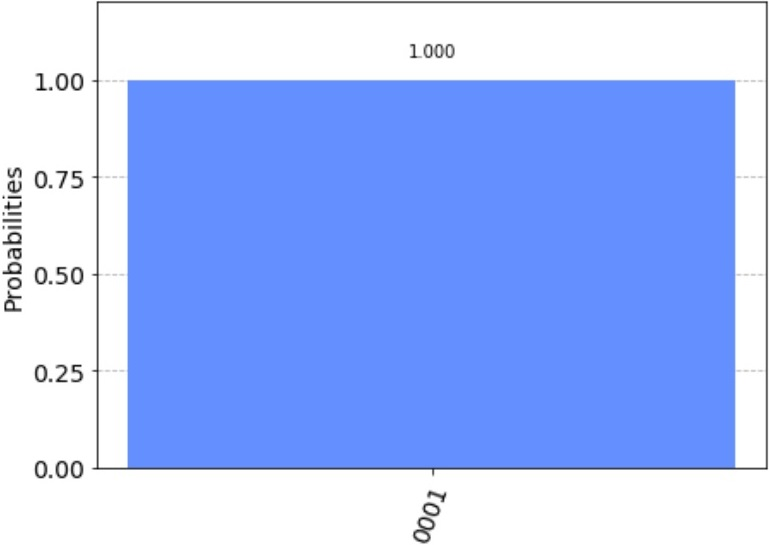
\includegraphics[width=1\textwidth]{../tex/images/simulator_balanced}
        Resultados con función balanceada en simulador.
    \end{minipage}\hfill
    \begin{minipage}{0.45\textwidth}
        \centering
        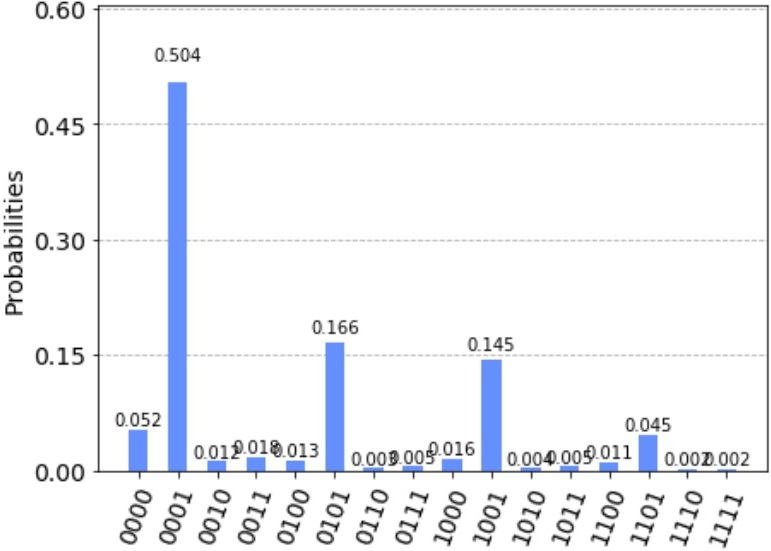
\includegraphics[width=1\textwidth]{../tex/images/ibmq_balanced}
        Resultados con función balanceada en ordenador cuántico de IBM.
    \end{minipage}
\end{figure}
\end{frame}

\begin{frame}
\frametitle{Evaluación del algoritmo}
Evaluación para $f\equiv1$ de 4 bits de entrada tras 1024 ejecuciones. 
\begin{figure}[htb!]
    \centering
    \begin{minipage}{0.45\textwidth}
        \centering
        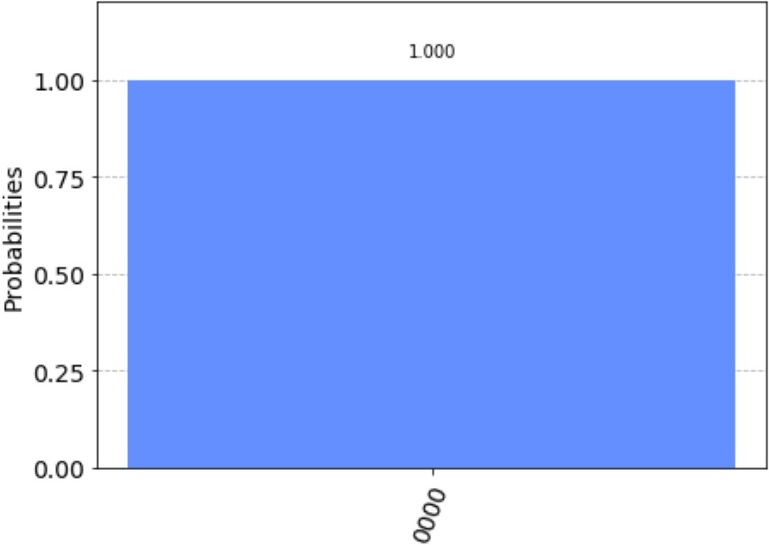
\includegraphics[width=1\textwidth]{../tex/images/simulator_constant}
        Resultados con función constante en simulador.
    \end{minipage}\hfill
    \begin{minipage}{0.45\textwidth}
        \centering
        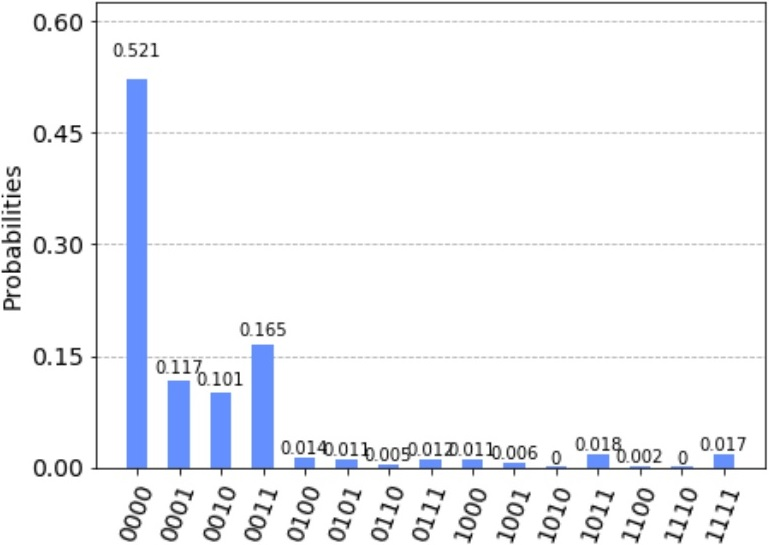
\includegraphics[width=1\textwidth]{../tex/images/ibmq_constant}
        Resultados con función constante en ordenador cuántico de IBM.
    \end{minipage}
\end{figure}
\end{frame}



\end{document}